


\usetikzlibrary{calc,through}
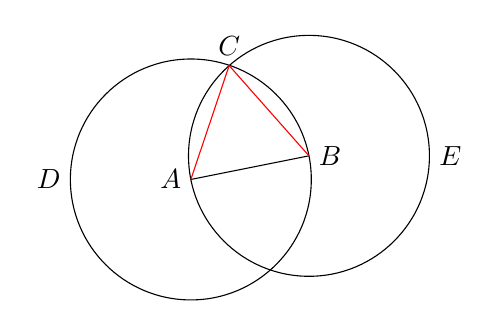
\begin{tikzpicture}[scale=1.2]
\coordinate [label=left:$A$] (A) at (0,0);
\coordinate [label=right:$B$] (B) at (1.25,0.25);
\draw (A) -- (B);
\node (D) [draw,circle through=(B),label=left:$D$] at (A) {};
\node (E) [draw,circle through=(A),label=right:$E$] at (B) {};
\coordinate[label=above:$C$] (C) at (intersection 2 of D and E);
\draw [red] (A) -- (C);
\draw [red] (B) -- (C);
\end{tikzpicture}
